\subsection{Physiological Dangers}
Characters might find themselves without food, water, or sleep and with no means to obtain them.

Characters who have taken nonlethal damage from lack of food, water, or sleep, are fatigued. Nonlethal damage from dehydration, starvation, or sleep deprivation, cannot be recovered until the character gets food, water, or sleep, as needed---not even magic that restores hit points heals this damage.

A character with the \skill{Survival} skill can gather enough food and water with a check. Characters gathering resources travel at half their overland speed. See the table below for DCs and modifiers. A character can provide food and water for one other person for every number of points in Extra Person Modifier by which their check result exceeds the DC.

\Table{Get Along in the Wild}{X *{2}{Z{9mm}}}{
  \tableheader Terrains
& \tableheader Survival DC
& \tableheader Extra Person Modifier\\
Forests, lakes, oasis, oceans               & 10 & 2 \\
Verdant plains, swamp, mudflats             & 15 & 3 \\
Mountains, rocky badlands, scrub plains     & 20 & 5 \\
Boulder fields, sandy wastes, stony barrens & 25 & 7 \\
Dust sinks, salt flats, sea of silt         & 30 & 10 \\
Obsidian Plains                             & 40 & 15 \\
}

A character can also use the \skill{Survival} skill to find or make a shelter to protect from the sun to get some sleep. This does not remove the possibility of a random encounter, just make sure the character can get a good night of sleep. This process takes 1d4 hours.

\begin{figure}[t!]
\centering
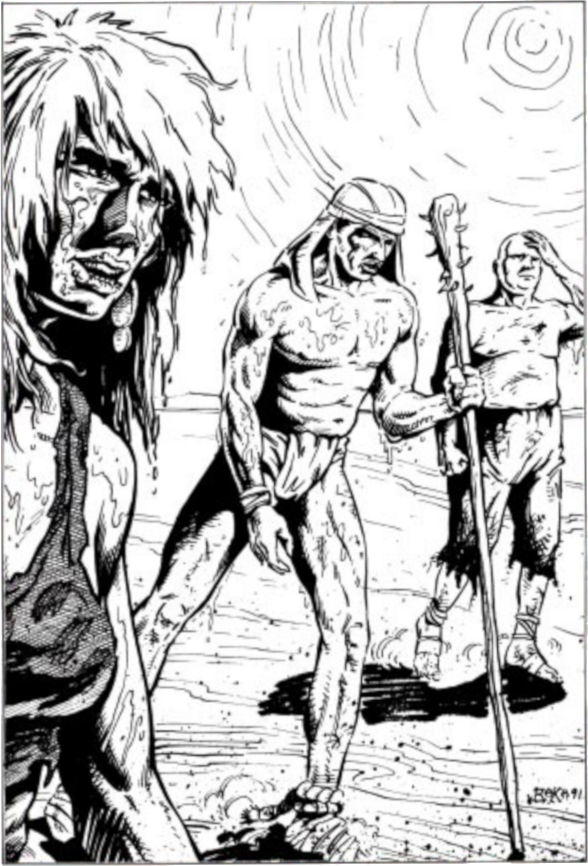
\includegraphics[width=\columnwidth]{images/dehydration.png}
\WOTC
\end{figure}

\Table{Find Shelter}{X Z{9mm}}{
\tableheader Terrains & \tableheader Survival DC \\
Forests, mountains, oasis, rocky badlands, scrub plains & 15 \\
Boulder fields, stony barrens, swamp                    & 20 \\
Verdant plains, mudflats                                & 25 \\
Obsidian Plains, salt flats                             & 20 \\
Dust sinks, sea of silt                                 & 30 \\
Lakes, oceans                                           & 40 \\
}

\subsubsection{Dehydration}
While in a temperate climate a character must consume 3 liters of water per day to avoid dehydration, the Tablelands are not so gentle.

In particularly hot environments (very hot or worse), characters need double the normal amount. The amount of water required to avoid dehydration increases by 3 liters per temperature band higher than very hot (so 6 liters in severe heat, 9 liters in extreme heat, and so on). \tabref{Water Per Day} indicates how many liters are needed during a typical day for all character sizes. Creatures that remain inactive (sitting, resting, or sleeping) need half that amount per day.

\Table{Water Per Day}{p{28mm}RRRR}{
& \multicolumn{4}{c}{\tableheader Weather (Temperature, Wind)}\\
\cmidrule[.5pt]{2-5}
  \tableheader Character Size
& \tableheader Normal, Calm
& \tableheader Normal, Strong
& \tableheader Hot, Calm
& \tableheader Hot, Strong \\
Small and Medium    &  4 liters &  5 liters &  6 liters &  8 liters \\
Large (half-giants) & 16 liters & 20 liters & 24 liters & 32 liters \\
}

A creature can go without water for a number of hours equal to 24 + its Constitution score. After this time, the creature must make a successful Constitution check each hour (DC 10, +1 for each previous check) or take 1d6 points of nonlethal damage. Every full day without water after this time, the creature takes 1 point of Constitution damage. Characters who have taken any damage from lack of water are fatigued.

In particularly hot environments (very hot or worse), the time a creature can go without water before making Constitution checks is reduced. Each hour counts as one more hour per temperature band higher than very hot (so 2 hours in severe heat, 3 hours in extreme heat, and so on). See \tabref{Effective Hours Without Water} for reference of how many ``water hours'' are spend during each type of day. 

\Table{Effective Hours Without Water}{y{28mm}RRRR}{
& \multicolumn{4}{c}{\tableheader Weather (Temperature, Wind)}\\
\cmidrule[.5pt]{2-5}
& \tableheader Normal, Calm
& \tableheader Normal, Strong
& \tableheader Hot, Calm
& \tableheader Hot, Strong \\
Outside & 43 hours & 54 hours & 70 hours & 94 hours \\
Shelter & 24 hours & 24 hours & 24 hours & 29 hours \\
}

\textit{Muls:} Mul characters can go without water for a number of hours equal to 48 + twice their Constitution score. After this time, the mul must make a successful Constitution check every two hours (DC 10, +1 for each previous check) or take 1d6 points of nonlethal damage. Every two days without water after this time, the mul takes 1 point of Constitution damage. Muls need the same amount of water per day as a human.

\textit{Thri-kreens:} Thri-kreen characters can go without water for a number of days equal to 7 + their Constitution modifier. After this time, a thri-kreen must make a successful Constitution check every day (DC 10, +1 for each previous check) or take 1d6 points of nonlethal damage. Every week without water after this time, the thri-kreen takes 1 point of Constitution damage. Thri-kreens need the 4 liters of water per week. Thri-kreens are not affected by temperature for water usage purposes.

\textbf{Dehydrated:} Characters who have taken any damage from lack of water are considered dehydrated and become fatigued. In addition, if a dehydrated character would take nonlethal damage from hot conditions, that damage instead becomes lethal damage.

A character who falls unconscious from nonlethal damage due to thirst begins to take the same amount of lethal damage instead. Damage from thirst, whether lethal or nonlethal, cannot be recovered until the character has been treated; not even magic that restores hit points or ability damage heals this damage.

\textbf{Treating Dehydration:} A character who has taken nonlethal damage from lack of water must be treated with long-term care (see the \skill{Heal} skill description) to recover. This treatment requires 24 hours of care and double the normal amount of water required per day for the conditions (for instance, 6 liters of water in normal conditions). If the character has also taken lethal damage from lack of water or from a hot environment, add 5 to the \skill{Heal} DC and double the time required to recover (to 48 hours). Once this \skill{Heal} check has succeeded, the damage taken by the character can be restored through the normal means.

% Alternatively, certain spells can be used to rehydrate a character in place of the recovery time, water, and \skill{Heal} check. The \spell{heal} spell accomplishes this function.

\subsubsection{Starvation}
A character can go without food for 3 days, in growing discomfort. After this time, the character must make a Constitution check each day (DC 10, +1 for each previous check) or take 1d6 points of nonlethal damage. Every week without food after this time, the character takes 1 point of Strength and Constitution damage. Characters who have taken any damage from lack of food are fatigued.

Damage from hunger cannot be recovered until the character has been treated; not even magic that restores hit points or ability damage heals this damage.

\textit{Muls:} Mul characters can go without food for 6 days. After this time, the character must make a Constitution check every two days (DC 10, +1 for each previous check) or take 1d6 points of nonlethal damage. Every two weeks without food after this time, the character takes 1 point of Strength and Constitution damage.

\textbf{Refeeding Syndrome:} A starving character who starts feeding without treatment must make a successful Fortitude save (DC 15, +1 for each week without food) or die. Without treatment, a character's metabolic rate spikes and may cause heart failure.

\textbf{Treating Starvation:} A character who has taken nonlethal damage from lack of food must be treated with long-term care (see the \skill{Heal} skill description) to recover. This treatment requires 24 hours of care. Once this \skill{Heal} check has succeeded, the damage taken by the character can be restored through the normal means.

\subsubsection{Sleep Deprivation}
A living creature can go without sleep for a number of days equal to its Constitution modifier (minimum one). After this time, a number of conditions happen:
\begin{itemize*}
\item Every four hours, the character must make a Will save (DC 10, +1 for each previous save) or fall asleep. On a success, the character takes 1 point of nonlethal damage. Characters who have taken nonlethal damage from lack of sleep are fatigued.
\item Each day after that period, the creature takes 1 point of Intelligence and Wisdom damage. This damage cannot be recovered until the character sleeps.
\end{itemize*}

Nonlethal damage from lack of sleep cannot be recovered until the character has slept. The \spell{sleep} or \spell{deep slumber} spells can help. If the total Wisdom damage exceeds its Hit Dice, the creature acts as if affected by the \spell{confusion} spell. Once any mental ability score drops to 0, the creature drops into a deep sleep for one whole day. (Attribute damage is healed normally in this sleep.)

\textit{Muls:} Mul characters can go without sleep for a number of days equal to twice their Constitution modifier (minimum two).

\textit{Thri-kreens:} Thri-kreen characters do not sleep and are not affected by the humanoid restrictions of sleep. They do need to rest 8 hours to prepare spells.

\textbf{Poor Sleep:} Characters that need sleep may need to do so under poor conditions, such as under the scorching sun. Under such conditions, characters do not heal ability damage and do not get the mental rest needed to prepare spells or regain power points. They regain half the amount of hit points as normal. They become fatigued for the rest of the day, or until they get a good sleep. Note that this poor sleep does not count as ``not sleeping''---a poor sleep is better than no sleep at all.